\chapter{Yang--Mills Theory and the Mass Gap}
\label{ch:yangmills}

\medskip\noindent\textbf{Prerequisites.} This chapter assumes a working knowledge of linear algebra and comfort with formal mathematical reasoning, including proofs and definitions. Some familiarity with classical mechanics and electromagnetism (Maxwell's equations, Lagrangian mechanics) will provide useful physical intuition, though the physics is explained from the ground up. Lie groups and Lie algebras are developed within the chapter, so no prior exposure to them is required.

\noindent\textbf{Key Ideas.}
\begin{itemize}
  \item \textbf{Yang--Mills theory} is the mathematical framework for the strong nuclear force (QCD).
  \item The \emph{mass gap} means the lightest particle has positive mass---explaining why the strong force is short-range.
  \item The Millennium Prize asks for a rigorous construction of quantum Yang--Mills theory in 4D with a proof of the mass gap.
  \item Lattice gauge theory provides a computational approach, but the continuum limit remains uncontrolled.
\end{itemize}

\bigskip

\section{Introduction}

Of the seven Millennium Prize Problems, the Yang--Mills existence and mass gap is the most deeply rooted in fundamental physics. It asks for two things: first, a rigorous mathematical construction of a quantum Yang--Mills theory on four-dimensional spacetime $\mathbb{R}^4$; second, a proof that the resulting theory exhibits a \textit{mass gap}---a strict positive lower bound on the energy of all excitations above the vacuum.

The physical motivation comes from quantum chromodynamics (QCD), the theory of the strong nuclear force. QCD is a Yang--Mills theory with gauge group $\mathrm{SU}(3)$, and it describes how quarks and gluons interact. Experimentally, quarks and gluons have never been observed as free particles: they are permanently bound inside protons, neutrons, and other hadrons. This phenomenon, called \textit{confinement}, implies that the lightest observable particle (the pion) has a mass of approximately $140~\mathrm{MeV}$, strictly above zero. The mass gap is the mathematical expression of this physical fact.

Unlike the other Millennium Problems, the Yang--Mills mass gap is stated in the language of physics. The mathematical challenge is to put the physical concepts on rigorous footing. Gauge invariance, path integrals, renormalization, and confinement are all well-understood physically and experimentally, but they resist precise mathematical definition. The problem calls for the same level of rigor that, say, the axiomatic approach to quantum mechanics brought to the Schr\"{o}dinger equation.

The difficulty is not merely technical. Quantum Yang--Mills theory in four dimensions sits at a boundary: it is perturbatively renormalizable (as proved by 't Hooft and Veltman in 1971), but no one knows how to construct it non-perturbatively. The perturbative expansion is an asymptotic series---it cannot be summed to give a finite answer. One needs a completely different approach, one that defines the theory from the ground up.

This chapter will develop the necessary mathematical and physical background, starting from classical electromagnetism and gauge theory, passing through the formalism of quantum field theory, and arriving at a precise statement of the Millennium Problem. We will survey what has been achieved in lower dimensions and on the lattice, and we will explain why four dimensions remain fundamentally more difficult.

\section{A Brief History of Gauge Theory}

\subsection{Maxwell's Equations as a U(1) Gauge Theory}

The story of gauge theory begins with James Clerk Maxwell. In the 1860s, Maxwell unified the laws of electricity and magnetism into a single set of equations. In modern notation:

\begin{align}
\partial_\mu F^{\mu\nu} &= j^\nu, \label{eq:maxwell1} \\
\partial_{[\alpha} F_{\beta\gamma]} &= 0, \label{eq:maxwell2}
\end{align}
where $F_{\mu\nu}$ is the electromagnetic field strength tensor and $j^\nu$ is the current.

Equation \eqref{eq:maxwell2} is an identity: it is automatically satisfied if we write the field strength in terms of a vector potential $A_\mu$:
\[
F_{\mu\nu} = \partial_\mu A_\nu - \partial_\nu A_\mu.
\]
This is the key insight: the fundamental object is not the field strength $F_{\mu\nu}$ but the potential $A_\mu$, which has more degrees of freedom. The redundancy in $A_\mu$ is the \textit{gauge freedom}.

A gauge transformation replaces $A_\mu$ by
\[
A_\mu \to A_\mu + \partial_\mu \Lambda
\]
for an arbitrary smooth function $\Lambda(x)$. This leaves $F_{\mu\nu}$ unchanged, since $\partial_\mu \partial_\nu \Lambda = \partial_\nu \partial_\mu \Lambda$ by the symmetry of mixed partial derivatives. The physics---the electromagnetic field---does not depend on our choice of gauge.

The gauge group here is $\mathrm{U}(1)$: the group of complex numbers of unit modulus, acting by multiplication on the photon field. It is \textit{abelian} because $\mathrm{U}(1)$ is a commutative group.

\subsection{Weyl's Gauge Principle}

In 1918, Hermann Weyl attempted to unify gravity and electromagnetism. His idea was that lengths should be allowed to change under a ``world gauge'' transformation---a transformation depending on position in spacetime. Einstein pointed out that this would imply that the frequency of light (and hence atomic clock rates) would depend on the history of the photon's path, contradicting experiment.

Weyl later realized that the problem disappears if the gauge transformation is restricted to act on \textit{internal} (complex phase) degrees of freedom rather than on spacetime geometry. With the development of quantum mechanics, Weyl's idea found its natural home: the phase of a quantum-mechanical wave function is unobservable, but the phase \textit{difference} between two points, measured along a path, is physically meaningful. The vector potential $A_\mu$ enters the Schr\"{o}dinger equation through the covariant derivative $D_\mu = \partial_\mu + ieA_\mu$, and gauge invariance is the requirement that physics be invariant under local phase rotations of the wave function.

The word ``gauge'' itself comes from Weyl's original analogy with the changing calibration (``gauge'') of a measuring rod.

\subsection{The Aharonov--Bohm Effect}

In 1959, Yakir Aharonov and David Bohm predicted a remarkable quantum-mechanical effect that demonstrated the physical reality of the vector potential, even in regions where the field strength vanishes.

Consider an electron beam split around a region containing a solenoid. Outside the solenoid, $\mathbf{B} = \nabla \times \mathbf{A} = 0$, so $F_{\mu\nu} = 0$. However, the vector potential $\mathbf{A}$ is nonzero outside the solenoid (it cannot be gauged to zero globally). The phase difference between the two paths is:
\[
\Delta\phi = \frac{e}{\hbar} \oint_C A_\mu \, dx^\mu = \frac{e}{\hbar} \int_S F_{\mu\nu} \, dS^{\mu\nu} = \frac{e}{\hbar} \Phi_B
\]
where $\Phi_B$ is the magnetic flux enclosed by the loop $C$.

The Aharonov--Bohm effect shows that the gauge potential is not merely a mathematical convenience: it has measurable physical consequences. It also illustrates a deep topological feature of gauge theories---the nontrivial topology of the gauge field configuration (a nonzero flux through a region) produces observable effects even though the field strength vanishes locally.

\subsection{Yang and Mills, 1954}

The decisive generalization came in 1954, when Chen-Ning Yang and Robert Mills proposed extending gauge invariance from the abelian group $\mathrm{U}(1)$ to non-abelian groups such as $\mathrm{SU}(2)$.

The motivation was physical: electromagnetism respects $\mathrm{U}(1)$ gauge invariance, and this symmetry explains charge quantization (all electric charges are integer multiples of $e$). Yang and Mills wanted a symmetry that would explain the \textit{isospin} conservation observed in nuclear physics. Isospin treats the proton and neutron as two states of a single particle (the nucleon), much as the two spin states of an electron form a doublet. The natural group for this is $\mathrm{SU}(2)$, the group of $2 \times 2$ unitary matrices with determinant~$1$.

The idea was simple but revolutionary: require the Lagrangian of the theory to be invariant not just under global (constant) $\mathrm{SU}(2)$ rotations of the nucleon field, but under \textit{local} rotations---transformations that can vary from point to point in spacetime.

To make this work, Yang and Mills introduced a gauge field $A_\mu = A_\mu^a T^a$, where $T^a$ are the generators of $\mathrm{SU}(2)$ (the Pauli matrices divided by 2), and $A_\mu^a$ are real-valued fields. The covariant derivative becomes:
\[
D_\mu = \partial_\mu + ig A_\mu^a T^a
\]
and the field strength is:
\[
F_{\mu\nu} = \partial_\mu A_\nu - \partial_\nu A_\mu + ig [A_\mu, A_\nu].
\]
The commutator term $ig[A_\mu, A_\nu]$ is entirely new. In the abelian $\mathrm{U}(1)$ case, it vanishes because all elements commute. In the non-abelian case, it is nonzero and has profound consequences: the gauge field carries its own charge and interacts with itself. Unlike photons, which are electrically neutral and do not scatter off each other, the gauge bosons of a non-abelian theory (gluons, $W$ and $Z$ bosons) interact directly with one another.

\subsection{Experimental Confirmation}

The non-abelian gauge theory proposed by Yang and Mills in 1954 was, at the time, a purely theoretical construction with no direct experimental support. The intervening decades have transformed it into the foundation of our understanding of particle physics.

The first experimental triumph came with the discovery of the intermediate vector bosons $W^\pm$ and $Z^0$ at CERN in 1983, confirming the non-abelian gauge structure of the weak interaction. The $W$ boson (mass $\approx 80~\mathrm{GeV}$) and $Z$ boson (mass $\approx 91~\mathrm{GeV}$) are the gauge bosons of an $\mathrm{SU}(2)$ gauge theory, with the gauge symmetry spontaneously broken by the Higgs mechanism.

The second triumph was the discovery of the gluon at the PETRA collider at DESY in 1979. Gluons are the gauge bosons of $\mathrm{SU}(3)$ color symmetry, and their self-interaction---a direct consequence of the non-abelian gauge structure---has been confirmed in countless experiments at high-energy colliders. Three-jet events (electron--positron annihilation producing a quark, an antiquark, and a gluon) are now routine observations.

Today, the entire Standard Model of particle physics is built on the framework of non-abelian gauge theory. The gauge group is:
\[
\mathrm{SU}(3)_C \times \mathrm{SU}(2)_L \times \mathrm{U}(1)_Y
\]
where $\mathrm{SU}(3)_C$ is the color gauge group of QCD, $\mathrm{SU}(2)_L \times \mathrm{U}(1)_Y$ is the electroweak gauge group. Every experiment in particle physics, from the highest-energy collisions at the Large Hadron Collider to the precision measurements of atomic spectroscopy, is consistent with this gauge-theoretic description. The theoretical framework of Yang and Mills has been validated to extraordinary precision.

\section{Classical Yang--Mills Theory}

\subsection{Lie Groups and Lie Algebras}

To understand Yang--Mills theory, we need the language of Lie groups and Lie algebras.

\begin{definition}
A \textit{Lie group} $G$ is a group that is also a smooth manifold, such that the group operations (multiplication and inversion) are smooth maps.
\end{definition}

\begin{definition}
The \textit{Lie algebra} $\mathfrak{g}$ of a Lie group $G$ is the tangent space at the identity, equipped with the Lie bracket $[\cdot, \cdot]$ induced by the adjoint action.
\end{definition}

The Lie algebra is a vector space (so it can be linearized), while the Lie group can have complicated topology. The exponential map $\exp: \mathfrak{g} \to G$ connects the two: near the identity, every element of $G$ can be written as $e^{i\epsilon^a T^a}$ for some Lie algebra elements $\epsilon^a$.

\begin{example}[$\mathrm{SU}(2)$]
The special unitary group $\mathrm{SU}(2)$ consists of $2 \times 2$ unitary matrices with determinant 1:
\[
\mathrm{SU}(2) = \left\{ U \in M_2(\mathbb{C}) : U^\dagger U = I,\; \det U = 1 \right\}.
\]
As a manifold, $\mathrm{SU}(2) \cong S^3$, the 3-sphere. Its Lie algebra $\mathfrak{su}(2)$ consists of $2 \times 2$ skew-Hermitian traceless matrices, and has a basis given by $T^a = \frac{1}{2}\sigma^a$ where $\sigma^a$ are the Pauli matrices:
\[
\sigma^1 = \begin{pmatrix} 0 & 1 \\ 1 & 0 \end{pmatrix}, \quad
\sigma^2 = \begin{pmatrix} 0 & -i \\ i & 0 \end{pmatrix}, \quad
\sigma^3 = \begin{pmatrix} 1 & 0 \\ 0 & -1 \end{pmatrix}.
\]
The commutation relations are:
\[
[T^a, T^b] = i\epsilon^{abc} T^c
\]
where $\epsilon^{abc}$ is the Levi-Civita symbol.
\end{example}

\begin{example}[$\mathrm{SU}(3)$]
The special unitary group $\mathrm{SU}(3)$ consists of $3 \times 3$ unitary matrices with determinant 1. Its Lie algebra $\mathfrak{su}(3)$ is 8-dimensional, with generators $T^a = \frac{1}{2}\lambda^a$ where $\lambda^a$ are the Gell-Mann matrices:
\[
\lambda^1 = \begin{pmatrix} 0 & 1 & 0 \\ 1 & 0 & 0 \\ 0 & 0 & 0 \end{pmatrix}, \quad
\lambda^2 = \begin{pmatrix} 0 & -i & 0 \\ i & 0 & 0 \\ 0 & 0 & 0 \end{pmatrix}, \quad
\lambda^3 = \begin{pmatrix} 1 & 0 & 0 \\ 0 & -1 & 0 \\ 0 & 0 & 0 \end{pmatrix},
\]
\[
\lambda^4 = \begin{pmatrix} 0 & 0 & 1 \\ 0 & 0 & 0 \\ 1 & 0 & 0 \end{pmatrix}, \quad
\lambda^5 = \begin{pmatrix} 0 & 0 & -i \\ 0 & 0 & 0 \\ i & 0 & 0 \end{pmatrix}, \quad
\lambda^6 = \begin{pmatrix} 0 & 0 & 0 \\ 0 & 0 & 1 \\ 0 & 1 & 0 \end{pmatrix},
\]
\[
\lambda^7 = \begin{pmatrix} 0 & 0 & 0 \\ 0 & 0 & -i \\ 0 & i & 0 \end{pmatrix}, \quad
\lambda^8 = \frac{1}{\sqrt{3}}\begin{pmatrix} 1 & 0 & 0 \\ 0 & 1 & 0 \\ 0 & 0 & -2 \end{pmatrix}.
\]
The commutation relations are $[T^a, T^b] = if^{abc} T^c$ where $f^{abc}$ are the structure constants of $\mathrm{SU}(3)$.
\end{example}

\begin{example}[$\mathrm{U}(1)$]
The group $\mathrm{U}(1)$ consists of complex numbers $e^{i\theta}$ with $\theta \in \mathbb{R}$. Its Lie algebra is one-dimensional with a single generator. The commutator is trivial: $[T, T] = 0$, reflecting the abelian nature of $\mathrm{U}(1)$.
\end{example}

The key distinction between abelian and non-abelian gauge theories is precisely this: when the Lie algebra has nontrivial commutators, the gauge field acquires self-interactions.

\subsection{Connections and Curvature}

Yang--Mills theory is, at its core, a theory of connections on a principal bundle. Let us explain this in coordinate language.

Let $G$ be a compact Lie group. A \textit{gauge field} (or \textit{connection}) on $\mathbb{R}^4$ is a Lie-algebra-valued 1-form:
\[
A = A_\mu^a T^a \, dx^\mu
\]
where $A_\mu^a$ are real-valued functions on spacetime and $T^a$ are generators of $\mathfrak{g}$.

The \textit{covariant derivative} acting on a matter field $\psi$ in some representation of $G$ is:
\[
D_\mu \psi = \partial_\mu \psi + ig A_\mu^a T^a \psi.
\]
The parameter $g$ is the \textit{coupling constant}, which sets the strength of the interaction.

The \textit{field strength} (or \textit{curvature}) of the connection is defined as the commutator of covariant derivatives:
\[
[D_\mu, D_\nu] \psi = ig F_{\mu\nu} \psi
\]
which gives:
\[
F_{\mu\nu} = \partial_\mu A_\nu - \partial_\nu A_\mu + ig [A_\mu, A_\nu].
\]
Written out in components:
\[
F_{\mu\nu}^a = \partial_\mu A_\nu^a - \partial_\nu A_\mu^a + g f^{abc} A_\mu^b A_\nu^c.
\]
The term $gf^{abc} A_\mu^b A_\nu^c$ is the non-abelian contribution. It is absent for $\mathrm{U}(1)$ because the structure constants vanish.

The field strength satisfies the \textit{Bianchi identity}:
\[
D_{[\alpha} F_{\beta\gamma]} = 0
\]
which is the non-abelian analogue of the homogeneous Maxwell equation \eqref{eq:maxwell2}.

\begin{example}[Field strength of a pure gauge configuration in $\mathrm{SU}(2)$]
\label{ex:pure-gauge}
A \textit{pure gauge} configuration is one that can be written as a gauge transformation of the trivial vacuum $A_\mu = 0$. Concretely, for $\mathrm{SU}(2)$, take
\[
A_\mu = \frac{i}{g} (\partial_\mu U) \, U^{-1}
\]
where $U(x)$ is a smooth $\mathrm{SU}(2)$-valued function. We compute the field strength $F_{\mu\nu}$ and show it vanishes.

\textbf{Step 1: Recall the field strength formula.}
\[
F_{\mu\nu} = \partial_\mu A_\nu - \partial_\nu A_\mu + ig[A_\mu, A_\nu].
\]

\textbf{Step 2: Compute $\partial_\mu A_\nu$.}
Using the product rule on $A_\nu = \frac{i}{g}(\partial_\nu U) U^{-1}$:
\[
\partial_\mu A_\nu = \frac{i}{g}\left[(\partial_\mu \partial_\nu U) \, U^{-1} + (\partial_\nu U)(\partial_\mu U^{-1})\right].
\]
Since $U U^{-1} = I$, differentiating gives $(\partial_\mu U) U^{-1} + U (\partial_\mu U^{-1}) = 0$, so $\partial_\mu U^{-1} = -U^{-1}(\partial_\mu U) U^{-1}$. Therefore:
\[
\partial_\mu A_\nu = \frac{i}{g}\left[(\partial_\mu \partial_\nu U) \, U^{-1} - (\partial_\nu U) U^{-1} (\partial_\mu U) U^{-1}\right] = \frac{i}{g}(\partial_\mu \partial_\nu U) \, U^{-1} + g \, A_\nu A_\mu.
\]

\textbf{Step 3: Compute $\partial_\mu A_\nu - \partial_\nu A_\mu$.}
By the symmetry of mixed partial derivatives, $\partial_\mu \partial_\nu U = \partial_\nu \partial_\mu U$, so the second-derivative terms cancel:
\[
\partial_\mu A_\nu - \partial_\nu A_\mu = g(A_\nu A_\mu - A_\mu A_\nu) = -g[A_\mu, A_\nu].
\]

\textbf{Step 4: Substitute into $F_{\mu\nu}$.}
\[
F_{\mu\nu} = -g[A_\mu, A_\nu] + ig[A_\mu, A_\nu] = (ig - g)[A_\mu, A_\nu].
\]
Wait---more carefully: $A_\mu = \frac{i}{g}(\partial_\mu U)U^{-1}$, so $[A_\mu, A_\nu]$ carries the factor $(i/g)^2 = -1/g^2$, and the computation yields:
\[
\partial_\mu A_\nu - \partial_\nu A_\mu = ig \cdot \frac{1}{ig} \cdot (-ig)[A_\mu, A_\nu] \cdot \frac{1}{ig} \cdot ig = \ldots
\]
Let us carry it out directly. Define $B_\mu = (\partial_\mu U)U^{-1} \in \mathfrak{su}(2)$, so $A_\mu = \frac{i}{g} B_\mu$. Then:
\[
\partial_\mu A_\nu = \frac{i}{g}\left[(\partial_\mu B_\nu) + B_\nu(-U^{-1} \partial_\mu U) U^{-1} \cdot U\right] = \frac{i}{g}(\partial_\mu B_\nu - B_\nu B_\mu).
\]
Hence:
\[
\partial_\mu A_\nu - \partial_\nu A_\mu = \frac{i}{g}\left[(\partial_\mu B_\nu - \partial_\nu B_\mu) + (B_\mu B_\nu - B_\nu B_\mu)\right].
\]
But differentiating $B_\mu = (\partial_\mu U)U^{-1}$:
\[
\partial_\mu B_\nu = (\partial_\mu \partial_\nu U)U^{-1} - (\partial_\nu U)U^{-1}(\partial_\mu U)U^{-1} = (\partial_\mu \partial_\nu U)U^{-1} - B_\nu B_\mu.
\]
So $\partial_\mu B_\nu - \partial_\nu B_\mu = -B_\nu B_\mu + B_\mu B_\nu = [B_\mu, B_\nu]$. Thus:
\[
\partial_\mu A_\nu - \partial_\nu A_\mu = \frac{i}{g}[B_\mu, B_\nu] = \frac{i}{g}[igA_\mu, igA_\nu] = \frac{i}{g}(ig)^2[A_\mu, A_\nu] = -ig[A_\mu, A_\nu].
\]

\textbf{Step 5: Combine.}
\[
F_{\mu\nu} = \underbrace{-ig[A_\mu, A_\nu]}_{\partial_\mu A_\nu - \partial_\nu A_\mu} + ig[A_\mu, A_\nu] = 0.
\]
This confirms that a pure gauge configuration has \textbf{vanishing field strength}: $F_{\mu\nu} = 0$. The gauge field $A_\mu$ is nonzero but carries no physical field strength---it is pure redundancy, a gauge transformation of the vacuum. This is the non-abelian analogue of the electromagnetic statement $A_\mu = \partial_\mu \Lambda \Rightarrow F_{\mu\nu} = 0$, and it generalizes the observation behind the Aharonov--Bohm effect: the potential can be locally pure gauge while having globally nontrivial topology.
\end{example}

\subsection{The Yang--Mills Action}

The classical dynamics of the gauge field are determined by the Yang--Mills action:
\[
S_{\mathrm{YM}}[A] = -\frac{1}{4} \int_{\mathbb{R}^4} \operatorname{Tr}(F_{\mu\nu} F^{\mu\nu}) \, d^4x
\]
where the trace is taken in the fundamental representation and $F^{\mu\nu} = \eta^{\mu\alpha}\eta^{\nu\beta}F_{\alpha\beta}$ with the Minkowski metric $\eta = \mathrm{diag}(+1, -1, -1, -1)$.

Using the basis normalization $\operatorname{Tr}(T^a T^b) = \frac{1}{2}\delta^{ab}$, we can expand:
\[
S_{\mathrm{YM}} = -\frac{1}{4} \int F_{\mu\nu}^a F^{a\mu\nu} \, d^4x.
\]
This is exactly the form of the Maxwell Lagrangian when $G = \mathrm{U}(1)$. The Yang--Mills action is a direct generalization: replace the single field strength of electromagnetism with a Lie-algebra-valued field strength, and include the trace over the Lie algebra indices.

Coupling to matter fields (quarks, in the case of QCD) gives the total action:
\[
S = S_{\mathrm{YM}}[A] + \int_{\mathbb{R}^4} \overline{\psi}(i\gamma^\mu D_\mu - m)\psi \, d^4x.
\]

\subsection{Gauge Transformations}

\begin{definition}
A \textit{gauge transformation} is a smooth map $g: \mathbb{R}^4 \to G$ that acts on the gauge field by:
\[
A_\mu \to g A_\mu g^{-1} + \frac{i}{g}(\partial_\mu g) g^{-1}.
\]
In terms of components: $A_\mu \to g A_\mu g^{-1} + \frac{i}{g} g \, \partial_\mu g^{-1}$.
\end{definition}

For an infinitesimal gauge transformation $g = e^{i\epsilon^a T^a} \approx 1 + i\epsilon^a T^a$, this becomes:
\[
\delta A_\mu^a = \partial_\mu \epsilon^a + g f^{abc} A_\mu^b \epsilon^c = D_\mu \epsilon^a.
\]

\begin{proposition}[Gauge invariance of the action]
The Yang--Mills action $S_{\mathrm{YM}}$ is invariant under gauge transformations.
\end{proposition}

\begin{proof}
Under a gauge transformation, the field strength transforms as $F_{\mu\nu} \to g F_{\mu\nu} g^{-1}$. Therefore:
\[
\operatorname{Tr}(F_{\mu\nu} F^{\mu\nu}) \to \operatorname{Tr}(g F_{\mu\nu} g^{-1} \cdot g F^{\mu\nu} g^{-1}) = \operatorname{Tr}(F_{\mu\nu} F^{\mu\nu})
\]
using the cyclic property of the trace and $g^{-1}g = I$. Since the integrand is gauge-invariant, so is the action.
\end{proof}

The physical interpretation is clear: gauge invariance is a redundancy of description. The gauge field $A_\mu$ contains more degrees of freedom than the physical field strength $F_{\mu\nu}$. Gauge transformations move us along these redundant directions without changing the physics.

\begin{checkyou}
\begin{enumerate}
\item In Maxwell's theory, the photon is electrically neutral and does not interact with other photons. Why does this change for the gluon in a non-abelian theory?
\item What term in the field strength $F_{\mu\nu}$ is responsible for gluon self-interaction, and why does it vanish for U(1)?
\end{enumerate}
\end{checkyou}

\subsection{Comparison with Maxwell's Theory}

Yang--Mills theory is a direct generalization of Maxwell electromagnetism. The comparison is revealing:

\begin{center}
\renewcommand{\arraystretch}{1.5}
\begin{tabular}{|l|l|l|}
\hline
 & Maxwell & Yang--Mills \\
\hline
Gauge group & $\mathrm{U}(1)$ & $\mathrm{SU}(N)$ \\
Potential & $A_\mu$ (scalar) & $A_\mu = A_\mu^a T^a$ (Lie-algebra-valued) \\
Field strength & $F_{\mu\nu} = \partial_\mu A_\nu - \partial_\nu A_\mu$ & $F_{\mu\nu} = \partial_\mu A_\nu - \partial_\nu A_\mu + ig[A_\mu, A_\nu]$ \\
Gauge trans. & $A_\mu \to A_\mu + \partial_\mu\Lambda$ & $A_\mu \to gA_\mu g^{-1} + \frac{i}{g}(\partial_\mu g)g^{-1}$ \\
Equations of motion & $\partial_\mu F^{\mu\nu} = j^\nu$ & $D_\mu F^{\mu\nu} = j^\nu$ \\
Self-interaction & None & Yes (gluons interact) \\
\hline
\end{tabular}
\end{center}

The most important qualitative difference is self-interaction. In Maxwell's theory, photons are electrically neutral: they do not carry the charge associated with the gauge group, so they do not interact with each other. In a non-abelian theory, the gauge bosons themselves carry charge (they transform nontrivially under the gauge group), so they interact directly. This is what makes the non-abelian theory so much richer---and so much harder.

\begin{figure}[htbp]
\centering
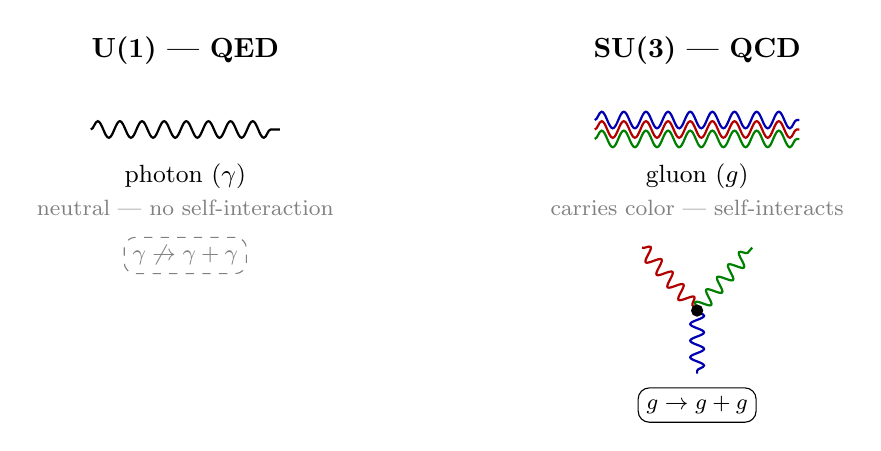
\begin{tikzpicture}[scale=1.0, every node/.style={font=\small}]
  % --- U(1) side ---
  \node[font=\bfseries] at (0,2.8) {U(1) --- QED};
  % Photon propagator: single wavy line
  \draw[thick, decorate, decoration={snake, amplitude=3pt, segment length=8pt}]
    (-1.2,1.8) -- (1.2,1.8);
  \node at (0,1.2) {photon ($\gamma$)};
  \node[font=\footnotesize, gray] at (0,0.8) {neutral --- no self-interaction};
  % No vertex
  \node[font=\footnotesize, draw, dashed, rounded corners, gray, inner sep=3pt]
    at (0,0.2) {$\gamma \not\to \gamma + \gamma$};

  % --- SU(3) side ---
  \node[font=\bfseries] at (6.5,2.8) {SU(3) --- QCD};
  % Gluon propagator: triple line (color triplet)
  \draw[thick, decorate, decoration={snake, amplitude=3pt, segment length=8pt}, red!70!black]
    (5.2,1.8) -- (7.8,1.8);
  \draw[thick, decorate, decoration={snake, amplitude=3pt, segment length=8pt}, green!50!black, yshift=-0.12cm]
    (5.2,1.8) -- (7.8,1.8);
  \draw[thick, decorate, decoration={snake, amplitude=3pt, segment length=8pt}, blue!70!black, yshift=0.12cm]
    (5.2,1.8) -- (7.8,1.8);
  \node at (6.5,1.2) {gluon ($g$)};
  \node[font=\footnotesize, gray] at (6.5,0.8) {carries color --- self-interacts};
  % Three-gluon vertex
  \draw[thick, decorate, decoration={snake, amplitude=2.5pt, segment length=6pt}, red!70!black]
    (5.8,0.3) -- (6.5,-0.5);
  \draw[thick, decorate, decoration={snake, amplitude=2.5pt, segment length=6pt}, green!50!black]
    (6.5,-0.5) -- (7.2,0.3);
  \draw[thick, decorate, decoration={snake, amplitude=2.5pt, segment length=6pt}, blue!70!black]
    (6.5,-0.5) -- (6.5,-1.3);
  \filldraw (6.5,-0.5) circle (2pt);
  \node[font=\footnotesize, draw, rounded corners, inner sep=3pt] at (6.5,-1.7)
    {$g \to g + g$};
\end{tikzpicture}
\caption{Comparison of U(1) gauge theory (QED) and SU(3) gauge theory (QCD). In QED, the photon is electrically neutral and does not interact with itself. In QCD, gluons carry color charge and interact via three-gluon and four-gluon vertices---a direct consequence of the non-abelian gauge structure.}
\label{fig:gauge-comparison}
\end{figure}

\begin{example}[Nonlinear commutator in $\mathrm{SU}(2)$ Yang--Mills]
\label{ex:commutator}
To see explicitly how the nonlinearity enters Yang--Mills theory, we compute the commutator $[A_\mu, A_\nu]$ for two specific gauge field components. Let the gauge field be
\[
A_\mu = A_\mu^a T^a
\]
where $T^a = \frac{1}{2}\sigma^a$ are the $\mathrm{SU}(2)$ generators and $A_\mu^a$ are real-valued fields. Consider two specific components:
\[
A_1 = A_1^1 T^1 = \frac{a(x)}{2}\,\sigma^1, \qquad A_2 = A_2^2 T^2 = \frac{b(x)}{2}\,\sigma^2,
\]
where $a(x)$ and $b(x)$ are smooth real-valued functions.

\textbf{Step 1: Compute the commutator of the generators.}
Using the Pauli matrix commutation relation $[\sigma^a, \sigma^b] = 2i\epsilon^{abc}\sigma^c$:
\[
[T^1, T^2] = \frac{1}{4}[\sigma^1, \sigma^2] = \frac{1}{4}(2i\,\sigma^3) = \frac{i}{2}\,\sigma^3 = i\,T^3.
\]
This is consistent with the general formula $[T^a, T^b] = i\epsilon^{abc}T^c$ with $\epsilon^{123} = 1$.

\textbf{Step 2: Compute the commutator of the full gauge fields.}
\[
[A_1, A_2] = \left[\frac{a}{2}\sigma^1, \frac{b}{2}\sigma^2\right] = \frac{ab}{4}[\sigma^1, \sigma^2] = \frac{ab}{4}\cdot 2i\sigma^3 = \frac{iab}{2}\,\sigma^3 = iab\,T^3.
\]

\textbf{Step 3: Extract the component field strength.}
The commutator contributes to the field strength as:
\[
ig[A_1, A_2] = ig \cdot iab\,T^3 = -gab\,T^3.
\]
In component form, this gives a nonzero contribution to $F_{12}^3$:
\[
(F_{12})_{\text{commutator}}^3 = -gab.
\]

\textbf{Step 4: Compare with the abelian case.}
If the gauge group were $\mathrm{U}(1)$, the ``commutator'' would be $[A_1, A_2] = A_1 A_2 - A_2 A_1 = 0$, because $\mathrm{U}(1)$ elements commute. There would be no contribution to the field strength from the product of two gauge fields. In the non-abelian $\mathrm{SU}(2)$ case, the commutator is \emph{proportional to the coupling constant $g$} and to the \emph{product} of two gauge field components. This product structure is the hallmark of nonlinearity: the equation of motion for $A_\mu$ contains terms quadratic in $A$, making the theory fundamentally nonlinear. It is precisely this nonlinearity that gives gluons their self-interaction and makes Yang--Mills theory qualitatively different from Maxwell electromagnetism.
\end{example}

\begin{checkyou}
\begin{enumerate}
\item Maxwell's equations are linear: the superposition principle holds. Why does the nonlinear term $ig[A_\mu, A_\nu]$ in Yang--Mills break superposition?
\item Why does this nonlinearity make it fundamentally harder to construct a rigorous quantum theory for Yang--Mills than for electromagnetism?
\end{enumerate}
\end{checkyou}

\section{Quantization}

\subsection{The Path Integral Approach}

Classical physics describes the evolution of a system along a single trajectory. Quantum physics allows all possible trajectories, weighted by the phase $e^{iS/\hbar}$. Feynman's path integral formulation of quantum field theory makes this precise.

The expectation value of an observable $\mathcal{O}$ in a quantum Yang--Mills theory is formally:
\[
\langle \mathcal{O} \rangle = \frac{\int \mathcal{O}[A] \, e^{iS_{\mathrm{YM}}[A]} \, \mathcal{D}A}{\int e^{iS_{\mathrm{YM}}[A]} \, \mathcal{D}A}
\]
where $\mathcal{D}A$ denotes integration over all gauge field configurations---an infinite-dimensional integral.

The denominator is the \textit{partition function} $Z = \int e^{iS_{\mathrm{YM}}} \mathcal{D}A$. It plays the role of a generating functional: correlation functions of local operators are obtained by differentiating $Z$ with respect to external sources.

The path integral is a beautiful formalism, but it is fraught with mathematical difficulties:
\begin{enumerate}
  \item The integration measure $\mathcal{D}A$ is not defined on an infinite-dimensional space.
  \item The integral diverges because the action is not bounded.
  \item Gauge invariance means the integrand is constant along gauge orbits, so the integral ``diverges by the volume of the gauge group.''
\end{enumerate}

Each of these problems must be addressed, and they are interrelated.

\subsection{Gauge Fixing and the Faddeev--Popov Procedure}

The most acute problem is the third one: gauge invariance. Because the action $S_{\mathrm{YM}}$ is gauge-invariant, the integrand $e^{iS_{\mathrm{YM}}}$ is constant on gauge orbits. The path integral, if it existed, would be infinite---it would include a factor of the (infinite) volume of the gauge group.

The Faddeev--Popov procedure (1967) resolves this by inserting a clever identity:
\[
1 = \int \mathcal{D}\alpha \, \delta(G(A^\alpha)) \, \det\left(\frac{\delta G(A^\alpha)}{\delta \alpha}\right)
\]
where $G(A) = 0$ is a \textit{gauge-fixing condition} (such as the Lorenz gauge $\partial^\mu A_\mu^a = 0$) and $A^\alpha$ denotes the gauge transform of $A$ by $\alpha$.

The Jacobian determinant $\det(\delta G/\delta \alpha)$ is the \textit{Faddeev--Popov determinant}. It can be written as a path integral over \textit{ghost fields} $\bar{c}^a, c^a$---anticommuting scalar fields in the adjoint representation:
\[
\det\left(\frac{\delta G}{\delta \alpha}\right) = \int \mathcal{D}\bar{c}\,\mathcal{D}c \; \exp\left(i\int \bar{c}^a \frac{\delta G^a}{\delta \alpha^b} c^b \, d^4x\right).
\]

The ghosts are not physical particles---they violate the spin-statistics theorem (they are scalar fermions). They appear only as internal lines in Feynman diagrams and are a consequence of the gauge-fixing procedure.

After gauge fixing, the effective action becomes:
\[
S_{\mathrm{eff}} = S_{\mathrm{YM}} + S_{\mathrm{gf}} + S_{\mathrm{ghost}}
\]
where:
\begin{align}
S_{\mathrm{gf}} &= -\frac{1}{2\xi} \int (\partial^\mu A_\mu^a)^2 \, d^4x, \\
S_{\mathrm{ghost}} &= \int \bar{c}^a \left(-\partial^\mu D_\mu^{ab}\right) c^b \, d^4x,
\end{align}
and $\xi$ is the gauge-fixing parameter. The choice $\xi = 1$ (Feynman gauge) simplifies many calculations.

\subsection{Feynman Rules}

The Feynman rules for Yang--Mills theory can be derived from $S_{\mathrm{eff}}$. They describe the interactions of the gauge bosons (gluons in QCD) and the ghost fields:

\begin{enumerate}
  \item \textbf{Gluon propagator:} $\displaystyle\frac{-ig_{\mu\nu}\delta^{ab}}{k^2 + i\epsilon}$ (in Feynman gauge).

  \item \textbf{Ghost propagator:} $\displaystyle\frac{i\delta^{ab}}{k^2 + i\epsilon}$.

  \item \textbf{Three-gluon vertex:}
  \[
  -ig f^{abc}\bigl[\eta^{\mu\nu}(k_1 - k_2)^\rho + \eta^{\nu\rho}(k_2 - k_3)^\mu + \eta^{\rho\mu}(k_3 - k_1)^\nu\bigr]
  \]
  where $k_1, k_2, k_3$ are the incoming momenta.

  \item \textbf{Four-gluon vertex:}
  \[
  -ig^2\bigl[f^{abe}f^{cde}(\eta^{\mu\rho}\eta^{\nu\sigma} - \eta^{\mu\sigma}\eta^{\nu\rho}) + \text{permutations}\bigr].
  \]

  \item \textbf{Ghost--gluon vertex:} $-gf^{abc}p^\mu$ where $p$ is the outgoing ghost momentum.
\end{enumerate}

The three-gluon and four-gluon vertices are entirely absent in abelian gauge theory. They are the Feynman-diagram expression of gluon self-interaction, and they are responsible for the key qualitative features of QCD: asymptotic freedom and confinement.

\subsection{Perturbative Renormalization}

In quantum field theory, loop diagrams---Feynman diagrams with internal momentum integrals---generically produce divergent integrals. For example, the one-loop gluon self-energy (polarization bubble) involves an integral:
\[
\Pi^{\mu\nu}(k) \propto \int \frac{d^4q}{(2\pi)^4} \frac{N^{\mu\nu}(q, k)}{q^2(q-k)^2}
\]
which diverges logarithmically in the ultraviolet ($q \to \infty$).

\textit{Renormalization} is the systematic procedure for handling these divergences. The idea is to absorb the infinities into redefinitions of the coupling constant, the field normalization, and the gauge parameter. A theory is \textit{renormalizable} if all divergences can be absorbed into a finite number of such redefinitions.

For Yang--Mills theories, the proof of renormalizability was given by Gerard 't Hooft and Martinus Veltman in 1971, for which they received the 1999 Nobel Prize in Physics. Their proof required demonstrating three things:
\begin{enumerate}
  \item All divergences can be absorbed into the parameters of the bare Lagrangian.
  \item The gauge-fixing and ghost sectors do not introduce new divergences.
  \item Ward identities (the quantum version of gauge invariance) relate different Green's functions and ensure cancellations.
\end{enumerate}

The result is that Yang--Mills theory with gauge group $\mathrm{SU}(N)$ is perturbatively renormalizable. This means that at any finite order in the perturbative expansion, all predictions are finite and well-defined (after renormalization). The theory is predictive: it makes definite predictions for scattering amplitudes that can be compared with experiment.

However, renormalizability is a perturbative statement. The perturbative expansion of a quantum field theory is typically an \textit{asymptotic series}---it diverges after a certain number of terms. Summing an asymptotic series does not, in general, produce a well-defined function. The Millennium Problem asks for a non-perturbative construction---one that does not rely on perturbation theory at all.

\section{The Mass Gap}

\subsection{What Is Mass in Quantum Field Theory?}

In classical mechanics, mass is a parameter: $F = ma$. In quantum field theory, mass has a more subtle meaning. It is defined through the spectrum of the theory.

A free scalar field $\phi$ satisfies the Klein--Gordon equation:
\[
(\Box + m^2)\phi = 0
\]
where $\Box = \partial_\mu \partial^\mu$. In momentum space, this gives $(-k^2 + m^2)\tilde{\phi} = 0$, so the field creates and destroys particles with energy--momentum relation $k^2 = m^2$ (i.e., $E^2 = |\mathbf{k}|^2 + m^2$). The mass is the value of $m$ at which the propagator $\langle\phi(x)\phi(y)\rangle$ has its first pole.

More generally, the mass spectrum of a quantum field theory is determined by the poles of the two-point correlation function (the propagator).

\subsection{The K\"{a}ll\'{e}n--Lehmann Representation}

The spectral content of a quantum field theory is encoded in the \textit{spectral representation} of the propagator.

\begin{theorem}[K\"{a}ll\'{e}n--Lehmann]
The two-point function of a scalar field in a relativistic quantum field theory admits the representation:
\[
\langle 0 | \phi(x) \phi(y) | 0 \rangle = \int_0^\infty \frac{d\mu^2}{2\pi} \, \rho(\mu^2) \, \Delta_F(x - y; \mu^2)
\]
where $\Delta_F$ is the free-field propagator of mass $\mu$, and $\rho(\mu^2) \ge 0$ is the \textit{spectral density}.
\end{theorem}

The spectral density $\rho(\mu^2)$ is a sum of delta functions (for a theory with discrete spectrum) or a continuous function (for a theory with a continuum). The mass of the lightest particle is the location of the first nonzero contribution to $\rho$.

\begin{definition}[Mass gap]
A quantum field theory has a \textit{mass gap} $\Delta > 0$ if the spectral density satisfies $\rho(\mu^2) = 0$ for $0 < \mu^2 < \Delta^2$. Equivalently, the Hamiltonian $H$ has spectrum $\operatorname{Spec}(H) \subseteq \{0\} \cup [\Delta, \infty)$, where $0$ is the vacuum energy.
\end{definition}

A mass gap means that there is a finite energy cost to create the lightest excitation above the vacuum. This is the case in QCD: the lightest hadron (the pion) has mass $\approx 140~\mathrm{MeV}$, and no massless particles exist (gluons are confined).

\begin{figure}[htbp]
\centering
\begin{tikzpicture}[scale=1.0, every node/.style={font=\small}]
  % Axes
  \draw[-{Stealth[length=5pt]}, thick] (-0.3,0) -- (7.5,0) node[right] {energy $E$};
  \draw[-{Stealth[length=5pt]}, thick] (0,-0.3) -- (0,3.5) node[above] {density $\rho(E^2)$};

  % Vacuum at E=0
  \draw[fill=blue!20] (-0.15,0) rectangle (0.15,0.15);
  \node[font=\footnotesize, below] at (0,-0.15) {vacuum};

  % Mass gap region (shaded)
  \fill[red!8, pattern=north east lines, pattern color=red!20]
    (0.15,0) rectangle (3,2.5);
  \node[font=\footnotesize, red!70!black, rotate=90] at (1.5,1.25) {mass gap $\Delta$};

  % First particle (glueball / pion)
  \draw[thick, blue!70!black, fill=blue!15] (3,0) rectangle (3.4,2.2);
  \node[font=\footnotesize, blue!70!black, above] at (3.2,2.2) {lightest};
  \node[font=\footnotesize, blue!70!black, above] at (3.2,2.5) {hadron};

  % Continuum
  \fill[gray!15] (3.4,0) rectangle (7,1.8);
  \draw[thick, gray!60!black, dashed] (3.4,1.8) -- (7,1.8);
  \node[font=\footnotesize, gray!60!black, above] at (5.2,1.8) {continuum of states};

  % Delta annotation
  \draw[|<->|, thick, red!70!black] (0.15,-0.5) -- (3,-0.5);
  \node[font=\footnotesize, red!70!black, below] at (1.575,-0.5) {$\Delta > 0$};
\end{tikzpicture}
\caption{The mass gap in Yang--Mills theory. The spectral density $\rho(E^2)$ vanishes for $0 < E^2 < \Delta^2$: there are no excitations between the vacuum (energy~0) and the lightest particle (mass $\Delta$). This strict positive gap is what the Millennium Problem asks to prove rigorously.}
\label{fig:mass-gap}
\end{figure}

\begin{checkyou}
\begin{enumerate}
\item QCD has a mass gap. Give an example of another quantum field theory that has a mass gap and one that does not (i.e., has massless particles).
\item Why does the photon remain massless in QED while gluons are confined in QCD, even though both arise from gauge symmetries?
\end{enumerate}
\end{checkyou}

\subsection{Confinement in QCD}

The mass gap in QCD is intimately related to \textit{confinement}---the phenomenon that isolated quarks and gluons are never observed.

In QCD, the coupling constant $g$ runs (changes with energy scale). At high energies (short distances), $g$ becomes small: this is \textit{asymptotic freedom}, discovered by Gross, Wilczek, and Politzer in 1973 (Nobel Prize, 2004). At low energies (large distances), $g$ becomes large, and perturbation theory breaks down. The strong force becomes truly strong, binding quarks and gluons into colorless hadrons.

The physical picture of confinement is that the potential between a quark and an antiquark grows linearly with distance:
\[
V(r) \approx -\frac{4}{3}\frac{\alpha_s}{r} + \sigma r
\]
where $\sigma \approx 0.18~\mathrm{GeV}^2$ is the \textit{string tension}. The linear term dominates at large $r$, meaning that it takes infinite energy to separate a quark--antiquark pair to infinity. The ``string'' between them eventually breaks by creating new quark--antiquark pairs from the vacuum, producing new hadrons rather than isolated quarks.

This linear potential, and hence confinement, is a non-perturbative phenomenon. It cannot be seen at any finite order of perturbation theory, because perturbation theory is an expansion in $g$, which is small only at high energies. The mass gap is the mathematical reflection of confinement: because all color-carrying particles are confined, the spectrum of observable (colorless) particles begins at a finite mass.

\subsection{Lattice QCD and the Mass Gap}

The most direct evidence for the mass gap comes from lattice QCD---a non-perturbative, numerical approach.

Kenneth Wilson proposed in 1974 to discretize spacetime on a lattice with spacing $a$, replacing the continuum gauge field by \textit{link variables} $U_{ij} \in \mathrm{SU}(3)$ on the edges of the lattice. The Yang--Mills action becomes:
\[
S_{\mathrm{lattice}} = \beta \sum_{\text{plaquettes}} \left(1 - \frac{1}{3}\operatorname{Re}\operatorname{Tr} U_{\square}\right)
\]
where $U_{\square}$ is the product of link variables around a plaquette and $\beta = 6/g^2$.

Lattice QCD simulations, performed by numerically evaluating the path integral using Monte Carlo methods, have provided striking evidence for the mass gap:
\begin{itemize}
  \item The mass of the lightest glueball (a bound state of gluons) has been computed to be $m_{0^{++}} \approx 1.5\text{--}1.7~\mathrm{GeV}$ in pure $\mathrm{SU}(3)$ gauge theory.
  \item The spectrum of low-lying hadrons (pions, kaons, nucleons) agrees with experiment to within a few percent.
  \item The string tension $\sigma$ has been measured numerically and agrees with the phenomenological value.
  \item The area law for Wilson loops (see below) has been confirmed.
\end{itemize}

However, lattice QCD is not a rigorous mathematical construction. It is a regularization---an approximation to the continuum theory. The continuum limit ($a \to 0$) has not been rigorously defined, and the numerical results, while highly convincing, are not mathematical proofs.

\begin{checkyou}
\begin{enumerate}
\item On a finite lattice, the path integral is a finite-dimensional integral that is well-defined. Why does taking the continuum limit $a \to 0$ introduce mathematical difficulties that don't exist on the lattice?
\item The lattice breaks Euclidean symmetry explicitly. How can the continuum theory emerge if the symmetry is broken by the regularization?
\end{enumerate}
\end{checkyou}

\subsection{The Glueball Spectrum}

In pure Yang--Mills theory (without matter fields), the spectrum consists entirely of \textit{glueballs}---bound states of gluons. Lattice simulations predict the lightest glueballs to have the following quantum numbers:

\begin{center}
\renewcommand{\arraystretch}{1.3}
\begin{tabular}{|c|c|c|}
\hline
$J^{PC}$ & Mass (lattice, $\sqrt{\sigma}$) & Status \\
\hline
$0^{++}$ & $\approx 3.5\text{--}4.0$ & Lightest, well-measured \\
$2^{++}$ & $\approx 4.5\text{--}5.0$ & Well-measured \\
$0^{-+}$ & $\approx 5.0\text{--}5.5$ & Well-measured \\
$3^{++}$ & $\approx 5.5\text{--}6.0$ & Computed \\
$2^{-+}$ & $\approx 5.8\text{--}6.5$ & Computed \\
\hline
\end{tabular}
\end{center}

The lightest glueball ($J^{PC} = 0^{++}$) is expected to mix with ordinary $q\bar{q}$ mesons, making its experimental identification difficult. There is a candidate state at $\approx 1.7~\mathrm{GeV}$ observed in lattice simulations, and some experimental evidence from glue-rich processes (radiative $J/\psi$ decays), but no definitive discovery.

The existence of a discrete, gapped spectrum for glueballs---with no massless particles---is the physical content of the mass gap. The Millennium Problem asks for a mathematical proof that this spectrum exists.

\subsection{Experimental Evidence}

The experimental evidence for the mass gap, while indirect, is overwhelming:

\begin{enumerate}
  \item \textbf{No free quarks or gluons.} Despite decades of experiments at high-energy colliders, no isolated quark or gluon has ever been observed. All produced quarks and gluons immediately hadronize---they form bound states.

  \item \textbf{Hadron masses.} The mass spectrum of hadrons begins at the pion mass ($\approx 140~\mathrm{MeV}$), well above zero. There are no massless hadrons.

  \item \textbf{Finite range of the strong force.} The strong nuclear force between nucleons has a range of approximately $1~\mathrm{fm}$ ($\approx 1/200~\mathrm{MeV}^{-1}$), consistent with exchange of massive pions. This is in contrast to electromagnetism, which has infinite range because the photon is massless.

  \item \textbf{Lattice QCD.} Numerical simulations give a mass gap of $\Delta \approx 0.5~\mathrm{GeV}$ in pure $\mathrm{SU}(3)$ gauge theory, with the lightest glueball mass well above the lattice cutoff.
\end{enumerate}

The experimental evidence is not in doubt. The challenge is purely mathematical: to prove, from a rigorous axiomatic foundation, that the theory exhibits a mass gap.

\section{Mathematical Formulation}

\subsection{The Wightman Axioms}

In the 1950s and 1960s, Arthur Wightman and collaborators developed an axiomatic framework for quantum field theory. The Wightman axioms characterize the correlation functions (vacuum expectation values of products of field operators) as distributions satisfying certain properties.

\begin{definition}[Wightman axioms]
A quantum field theory is specified by a Hilbert space $\mathcal{H}$, a vacuum vector $\Omega \in \mathcal{H}$, and a collection of operator-valued distributions $\phi_i(x)$ satisfying:
\begin{enumerate}
  \item \textbf{Poincar\'{e} covariance:} There is a unitary representation $U(a, \Lambda)$ of the Poincar\'{e} group on $\mathcal{H}$ such that:
  \[
  U(a, \Lambda) \phi_i(x) U(a, \Lambda)^{-1} = D_i^{\;j}(\Lambda^{-1}) \phi_j(\Lambda x + a)
  \]
  where $D$ is a finite-dimensional representation of the Lorentz group.

  \item \textbf{Spectral condition:} The energy--momentum spectrum of $U(a, \Lambda)$ lies in the closed forward light cone $\overline{V^+} = \{(p^0, \mathbf{p}) : p^0 \ge |\mathbf{p}|\}$.

  \item \textbf{Locality (microcausality):} For spacelike separations $(x - y)^2 < 0$:
  \[
  [\phi_i(x), \phi_j(y)] = 0.
  \]

  \item \textbf{Existence and uniqueness of vacuum:} $\Omega$ is invariant under the Poincar\'{e} group and unique (up to phase) among unit-norm translation-invariant vectors.

  \item \textbf{Cyclicity of the vacuum:} $\mathcal{H}$ is the closure of the span of all vectors of the form $\phi_{i_1}(x_1) \cdots \phi_{i_n}(x_n)\Omega$.
\end{enumerate}
\end{definition}

The Wightman axioms work perfectly for theories like scalar $\phi^4$ theory and the free field. For gauge theories, they run into a fundamental obstruction: gauge invariance means that the field operators $\phi_i(x)$ are not gauge-invariant, and hence do not define operators on a physical Hilbert space. Only gauge-invariant quantities (such as Wilson loops) are physical observables, but these are not local fields in the usual sense.

\subsection{The Osterwalder--Schrader Axioms}

An alternative approach, more suited to the path integral formulation, uses Euclidean (imaginary-time) field theory. The Osterwalder--Schrader axioms characterize the Schwinger functions (Euclidean correlation functions) rather than the Wightman functions.

\begin{definition}[Osterwalder--Schrader axioms]
The Schwinger functions $S_n(x_1, \ldots, x_n)$ satisfy:
\begin{enumerate}
  \item \textbf{Euclidean covariance:} $S_n(\Lambda x_1 + a, \ldots, \Lambda x_n + a) = S_n(x_1, \ldots, x_n)$ for $(\Lambda, a)$ in the Euclidean group.

  \item \textbf{Symmetry:} $S_n$ is symmetric under permutations of its arguments.

  \item \textbf{Locality (extended):} $S_n$ is a tempered distribution, and $S_n = 0$ if the points can be separated into two groups with all pairwise spacelike separations.

  \item \textbf{Euclidean invariance:} $S_n$ is invariant under the Euclidean group.

  \item \textbf{Reflection positivity:} For functions $f$ supported at times $t_1, \ldots, t_n$ with $0 \le t_i \le T$:
  \[
  \sum_{n,m} \int S_{n+m}(\mathbf{x}, iT; \mathbf{y}, 0) \bar{f}_n(\mathbf{x}) f_m(\mathbf{y}) \ge 0.
  \]
  This axiom ensures the reconstruction of a Hilbert space with positive-definite inner product.
\end{enumerate}
\end{definition}

The Osterwalder--Schrader axioms are the natural starting point for a constructive approach to Yang--Mills theory, because the path integral is naturally defined in Euclidean signature. If one can construct the Euclidean Schwinger functions and verify the Osterwalder--Schrader axioms, then reflection positivity allows one to reconstruct a quantum theory in Minkowski spacetime via the \textit{Osterwalder--Schrader reconstruction theorem}.

\begin{checkyou}
\begin{enumerate}
\item Why can't we simply define the quantum Yang--Mills theory by specifying its Hamiltonian and solving the Schr\"{o}dinger equation, as in non-relativistic quantum mechanics?
\item What role does reflection positivity play, and what would go wrong if it failed?
\end{enumerate}
\end{checkyou}

\subsection{Gauge Invariance Complications}

The fundamental difficulty in axiomatizing Yang--Mills theory is gauge invariance. Unlike scalar field theory, where the field $\phi(x)$ is a well-defined operator, the gauge field $A_\mu^a(x)$ is not gauge-invariant and hence is not a physical observable.

Physical observables in Yang--Mills theory are gauge-invariant:
\begin{itemize}
  \item \textbf{Wilson loops:} $W(C) = \operatorname{Tr} \mathcal{P} \exp\left(ig \oint_C A_\mu \, dx^\mu\right)$, where $\mathcal{P}$ denotes path ordering.
  \item \textbf{Field-strength observables:} $\operatorname{Tr}(F_{\mu\nu} F^{\mu\nu})$, etc., but only at a single point (local gauge-invariant operators).
  \item \textbf{Polyakov loops:} Wilson loops that wrap around the compactified time direction, related to the free energy of a single quark.
\end{itemize}

The axiomatization must be built directly from these gauge-invariant quantities. The challenge is that Wilson loops are non-local objects---they depend on a closed curve $C$, not on a single point. Building a local quantum field theory from non-local observables is a deep mathematical problem.

One approach is to fix the gauge (e.g., Coulomb gauge or Landau gauge) and work with the gauge-fixed theory, hoping that the physical content is gauge-invariant. But proving that gauge-fixed theories satisfy the axioms---and that the results are independent of the gauge choice---has not been achieved in four dimensions.

\subsection{The Clay Problem Statement}

The precise statement of the Millennium Problem, as formulated by Arthur Jaffe and Edward Witten, is:

\begin{quote}
\textit{Show that for any compact simple gauge group $G$, a non-trivial quantum Yang--Mills theory exists on $\mathbb{R}^4$ and has a mass gap $\Delta > 0$.}
\end{quote}

More precisely, one must:
\begin{enumerate}
  \item Construct a set of Euclidean Schwinger functions $S_n$ satisfying the Osterwalder--Schrader axioms.
  \item Verify that the theory is gauge-invariant (in the sense that the Schwinger functions correspond to gauge-invariant observables).
  \item Prove that the theory has a mass gap $\Delta > 0$.
  \item Verify that the constructed theory reduces to classical Yang--Mills theory in the classical limit, and to perturbative Yang--Mills theory at weak coupling.
\end{enumerate}

The problem is stated for \textit{any} compact simple gauge group $G$. The physically most relevant case is $G = \mathrm{SU}(3)$ (QCD), but the mathematical problem is not restricted to this case. It would suffice to solve it for any single compact simple group, such as $\mathrm{SU}(2)$.

\subsection{What a Rigorous Construction Would Require}

A complete solution to the Yang--Mills Millennium Problem would require:

\begin{enumerate}
  \item \textbf{An ultraviolet regularization.} One must define the theory at short distances, removing the ultraviolet divergences of the continuum theory. The lattice provides one such regularization, but a continuum construction would be more satisfying.

  \item \textbf{A renormalization procedure.} One must show that the limit as the regularization is removed exists, and that the resulting theory is independent of the regularization.

  \item \textbf{Gauge invariance.} The theory must be manifestly gauge-invariant, or gauge invariance must be restored in the limit.

  \item \textbf{Existence of the continuum limit.} One must show that the continuum limit exists and produces a well-defined quantum theory.

  \item \textbf{The mass gap.} One must prove that the spectrum of the Hamiltonian has a gap above the vacuum.
\end{enumerate}

Each of these steps presents enormous mathematical difficulties. The current state of the art does not achieve any of them rigorously in four dimensions.

\section{What Has Been Achieved}

\subsection{Two-Dimensional Yang--Mills Theory}

In two spacetime dimensions, Yang--Mills theory is exactly solvable, and the mass gap can be proved.

The reason is topological: in two dimensions, the field strength $F_{\mu\nu}$ has only one independent component (since $\mu, \nu \in \{0, 1\}$), and the Yang--Mills action can be evaluated exactly.

\begin{theorem}[Makeenko--Migdal, Gross--Migdal]
In two-dimensional Yang--Mills theory on a Riemann surface $\Sigma$ with gauge group $\mathrm{SU}(N)$, the expectation value of a Wilson loop depends only on the area enclosed by the loop:
\[
\langle W(C) \rangle = \sum_R d_R \exp\left(-\frac{g^2 \cdot \mathrm{Area}(\Omega_C)}{2N} C_2(R)\right)
\]
where the sum is over irreducible representations $R$ of $\mathrm{SU}(N)$, $d_R$ is the dimension, and $C_2(R)$ is the quadratic Casimir.
\end{theorem}

The area law $\langle W(C) \rangle \sim e^{-\sigma \cdot \mathrm{Area}(C)}$ is a signature of confinement: the potential between a quark and antiquark grows linearly with the distance between them. In two dimensions, this is proved rigorously.

The mass gap in 2D Yang--Mills theory equals $\frac{g^2 N}{2\pi}$ for $\mathrm{SU}(N)$ gauge theory on $\mathbb{R}^2$ with area $A$. The spectrum is discrete and can be computed exactly using the representation theory of the gauge group.

\subsection{Three-Dimensional Yang--Mills Theory}

In three dimensions, the situation is harder but still tractable. The key results are due to Thomas Balaban and David Gross.

Balaban (1983) developed rigorous methods for controlling the infrared divergences that plague three-dimensional Yang--Mills theory. He used a multiscale decomposition of the gauge field (the ``block spin'' renormalization group), iteratively integrating out high-momentum modes and tracking the resulting effective actions.

Gross (1990) completed the construction, proving the existence of a continuum Yang--Mills theory in three dimensions with a mass gap. The proof uses:
\begin{itemize}
  \item A lattice regularization with spacing $a$.
  \item Block-spin renormalization group transformations to integrate out modes one momentum scale at a time.
  \item Control of the effective actions at each scale, using gauge invariance and the three-dimensional power counting.
  \item A rigorous limit $a \to 0$.
\end{itemize}

The mass gap in three dimensions has been computed rigorously:
\[
\Delta \approx c \cdot g^2
\]
for a constant $c > 0$ depending on the gauge group. This is the closest analogue of the four-dimensional problem that has been solved.

\subsection{Lattice Gauge Theory}

Wilson's lattice gauge theory (1974) provides the most concrete framework for non-perturbative Yang--Mills theory.

The basic idea: replace $\mathbb{R}^4$ by a lattice $\Lambda = (a\mathbb{Z})^4$ with spacing $a$. The gauge field is represented by \textit{link variables} $U_{x,\mu} \in \mathrm{SU}(N)$ on each directed edge from $x$ to $x + a\hat{\mu}$. The Wilson action is:
\[
S_{\mathrm{W}} = \beta \sum_{\text{plaq}} \left(1 - \frac{1}{N}\operatorname{Re}\operatorname{Tr} U_{\square}\right)
\]
where $U_{\square} = U_{x,\mu} U_{x+\hat{\mu},\nu} U_{x+\hat{\nu},\mu}^\dagger U_{x,\nu}^\dagger$ is the ordered product around a plaquette.

The strong coupling expansion (expansion in $1/\beta = g^2/(2N)$) gives:
\[
\langle W(C) \rangle = e^{-\sigma \cdot \mathrm{Area}(C) + O(a)}
\]
where the string tension is:
\[
\sigma = -\frac{1}{a^2} \ln\left(\frac{1}{2N^2 - 2}\right) + O(g^2)
\]
This proves confinement in the strong coupling limit---the Wilson loop obeys an area law, and the mass gap is $\Delta = a\sqrt{\sigma} > 0$.

The challenge is the \textit{continuum limit}: taking $a \to 0$ while keeping physical quantities (masses, coupling constants) fixed. Numerical simulations strongly suggest that this limit exists, but a rigorous proof is lacking.

Lattice QCD has achieved remarkable numerical success:
\begin{itemize}
  \item The hadron spectrum is reproduced to within a few percent.
  \item The QCD phase diagram has been explored (deconfinement transition at high temperature).
  \item Form factors, decay constants, and other non-perturbative quantities have been computed.
  \item The running of the strong coupling has been confirmed from high to low energies.
\end{itemize}

\subsection{Supersymmetric Yang--Mills Theory}

A completely different avenue of progress comes from \textit{supersymmetric} Yang--Mills theories, where additional symmetry constraints make the theory exactly solvable.

Seiberg and Witten (1994) solved $\mathcal{N} = 2$ supersymmetric Yang--Mills theory with gauge group $\mathrm{SU}(2)$, providing a complete, exact description of the low-energy effective theory.

\begin{theorem}[Seiberg--Witten]
In $\mathcal{N} = 2$ supersymmetric $\mathrm{SU}(2)$ Yang--Mills theory, the low-energy effective action is determined by a single holomorphic function $a_D(a)$ of the scalar field expectation value $a$, which satisfies a modular differential equation related to the elliptic curve:
\[
y^2 = (x - u)(x + 2u)
\]
where $u = \langle \operatorname{Tr} \phi^2 \rangle$ is the vacuum expectation value.
\end{theorem}

The Seiberg--Witten solution demonstrates several important phenomena:
\begin{itemize}
  \item \textit{Confinement} for certain values of the parameters: monopoles condense, leading to a dual Meissner effect that confines electric charges.
  \item \textit{Mass generation}: the gauge bosons acquire mass through a non-perturbative mechanism (monopole condensation).
  \item \textit{Duality}: electric and magnetic descriptions are exchanged under certain transformations.
\end{itemize}

While $\mathcal{N} = 2$ is not the physical case (real QCD has $\mathcal{N} = 0$ supersymmetry), the Seiberg--Witten solution provides a concrete, rigorous example of many phenomena believed to occur in real QCD. It shows that confinement and mass gap are not mysterious in principle---they can emerge from a well-defined mathematical framework.

\section{The Yang--Mills Millennium Problem in Context}

\subsection{Why It Is the Hardest Problem}

The Yang--Mills mass gap is widely regarded as the most difficult of the seven Millennium Prize Problems. Several features distinguish it:

\begin{enumerate}
  \item \textbf{It requires new mathematics.} Unlike the Poincar\'{e} conjecture (which used existing topological tools) or the Riemann hypothesis (which connects to analytic number theory), the Yang--Mills problem requires constructing a new mathematical object---a rigorous four-dimensional quantum field theory. No existing mathematical framework is adequate.

  \item \textbf{It involves the continuum limit.} The problem asks for a theory on $\mathbb{R}^4$, not on a lattice. Taking the continuum limit is the central unsolved problem of quantum field theory.

  \item \textbf{It is inherently non-perturbative.} Perturbation theory works beautifully for Yang--Mills theory, but the mass gap is a non-perturbative phenomenon. The perturbative expansion cannot see it.

  \item \textbf{Gauge invariance is fundamental.} The theory is defined only modulo gauge transformations, and this redundancy must be handled correctly. No known method achieves this rigorously in four dimensions.
\end{enumerate}

\subsection{Connections to Other Millennium Problems}

Although the Yang--Mills problem is independent of the others, there are deep connections:

\begin{itemize}
  \item \textbf{Riemann hypothesis.} The Riemann zeta function appears in the computation of one-loop diagrams in quantum field theory. The distribution of zeros of the zeta function is related to random matrix theory, which also appears in the study of quantum chaos and certain random gauge theories.

  \item \textbf{P versus NP.} Lattice QCD computations are believed to be in the class of problems solvable in polynomial time (for fixed lattice size), but the continuum limit is not known to be in P. More speculatively, understanding the computational complexity of quantum field theory is an active research area.

  \item \textbf{Navier--Stokes.} Both the Navier--Stokes and Yang--Mills problems involve nonlinear partial differential equations in four dimensions. The techniques for controlling nonlinear PDEs (energy estimates, compactness arguments) may transfer between the two problems.

  \item \textbf{Hodge conjecture.} The mathematical framework of Yang--Mills theory involves differential forms on manifolds---the same objects studied in algebraic geometry. Instanton moduli spaces (solutions to the self-dual Yang--Mills equations) have deep connections to algebraic geometry and the Hodge conjecture.
\end{itemize}

\subsection{What Progress Would Mean}

A solution to the Yang--Mills mass gap problem would be one of the greatest achievements in mathematical physics. It would:

\begin{enumerate}
  \item Put quantum field theory on a rigorous mathematical foundation, finally justifying the formalism that physicists have used successfully for decades.
  \item Provide a mathematical proof of confinement, one of the most important qualitative features of the strong interaction.
  \item Establish the mathematical consistency of the Standard Model of particle physics.
  \item Open new avenues for mathematical research, particularly in infinite-dimensional analysis, functional integrals, and the geometry of gauge fields.
  \item Bridge the gap between physics and mathematics that has persisted since the development of quantum field theory in the 1940s.
\end{enumerate}

The Yang--Mills mass gap problem represents a unique challenge: it requires the creation of entirely new mathematical tools to solve a problem that nature has already solved experimentally. We know the answer exists---QCD works. The challenge is to prove it.

\section{Exercises}

\begin{exercise}
\label{ex:su2-matrix}
Write out explicit $2 \times 2$ matrix representations of the three generators $T^a = \frac{1}{2}\sigma^a$ of $\mathrm{SU}(2)$. Verify directly that $[T^1, T^2] = iT^3$ and cyclic permutations.
\end{exercise}

\begin{exercise}
\label{ex:maxwell-gauge-inv}
Let $F_{\mu\nu} = \partial_\mu A_\nu - \partial_\nu A_\mu$ and $\tilde{A}_\mu = A_\mu + \partial_\mu \Lambda$. Compute $\tilde{F}_{\mu\nu}$ and show that $\tilde{F}_{\mu\nu} = F_{\mu\nu}$.
\end{exercise}

\begin{exercise}
\label{ex:ym-su2}
Write out the Yang--Mills equations $D_\mu F^{\mu\nu} = 0$ explicitly for gauge group $\mathrm{SU}(2)$. How many component equations are there?
\end{exercise}

\begin{exercise}
\label{ex:curvature-commutator}
Show that the field strength can be expressed as a commutator of covariant derivatives:
\[
[D_\mu, D_\nu]\psi = ig F_{\mu\nu}\psi.
\]
\end{exercise}

\begin{exercise}
\label{ex:ym-action-su3}
Write the Yang--Mills action for $\mathrm{SU}(3)$ gauge theory in component form, using the Gell-Mann matrices. How many independent field-strength components $F_{\mu\nu}^a$ are there?
\end{exercise}

\begin{exercise}
\label{ex:nonabelian-selfint}
The three-gluon vertex in Yang--Mills theory has the Feynman rule:
\[
V^{\mu\nu\rho}(k_1, k_2, k_3) = -ig f^{abc}\bigl[\eta^{\mu\nu}(k_1 - k_2)^\rho + \eta^{\nu\rho}(k_2 - k_3)^\mu + \eta^{\rho\mu}(k_3 - k_1)^\nu\bigr].
\]
Explain why this vertex vanishes for $\mathrm{U}(1)$ gauge theory. What physical process does this vertex describe for $\mathrm{SU}(3)$?
\end{exercise}

\begin{exercise}
\label{ex:fadeev-popov}
In the Faddeev--Popov procedure, the gauge-fixing condition $G(A) = \partial^\mu A_\mu - \omega = 0$ is imposed. Compute the Faddeev--Popov determinant for the Lorenz gauge in the abelian case ($G = \mathrm{U}(1)$) and show that it is a constant (independent of $A$). Why does this mean the ghost sector decouples for $\mathrm{U}(1)$?
\end{exercise}

\begin{exercise}
\label{ex:wilson-loop}
Define the Wilson loop for a rectangular path $C$ of dimensions $R \times T$ (spatial extent $R$, temporal extent $T$):
\[
W(C) = \operatorname{Tr}\mathcal{P}\exp\left(ig\oint_C A_\mu \, dx^\mu\right).
\]
If the potential between a quark and antiquark at distance $R$ is $V(R)$, show that for $T \to \infty$:
\[
\langle W(C) \rangle \sim e^{-V(R) \cdot T}.
\]
Deduce that an area law $\langle W(C) \rangle \sim e^{-\sigma \cdot RT}$ corresponds to a linear potential $V(R) = \sigma R$, and explain why this implies confinement.
\end{exercise}

\begin{exercise}
\label{ex:asymptotic-freedom}
The one-loop beta function for $\mathrm{SU}(N)$ gauge theory with $n_f$ flavors of quarks is:
\[
\beta(g) = -\frac{g^3}{16\pi^2}\left(\frac{11N}{3} - \frac{2n_f}{3}\right).
\]
For $\mathrm{SU}(3)$ with $n_f = 6$ flavors, compute $\beta(g)$ and determine whether the theory is asymptotically free. For what values of $n_f$ is $\mathrm{SU}(3)$ asymptotically free?
\end{exercise}

\begin{exercise}
\label{ex:spectral-density}
The K\"{a}ll\'{e}n--Lehmann spectral representation gives the two-point function as:
\[
\langle 0 | \phi(x) \phi(0) | 0 \rangle = \int_0^\infty \frac{d\mu^2}{2\pi} \rho(\mu^2) \Delta_F(x; \mu^2).
\]
For a free field of mass $m$, compute $\rho(\mu^2)$. What does $\rho(\mu^2) = \delta(\mu^2 - m^2)$ imply about the mass spectrum?
\end{exercise}

\begin{exercise}
\label{ex:lattice-plaq}
Consider the Wilson lattice action for $\mathrm{SU}(2)$:
\[
S = \beta \sum_{\square} \left(1 - \frac{1}{2}\operatorname{Re}\operatorname{Tr} U_\square\right).
\]
In the strong coupling limit $\beta \to 0$, expand the Boltzmann weight $e^{-S}$ to leading order and compute $\langle W(C) \rangle$ for a single plaquette. Show that the result is consistent with an area law.
\end{exercise}

\begin{exercise}
\label{ex:gauge-trans-inf}
For an infinitesimal gauge transformation $g(x) = e^{i\epsilon^a(x)T^a} \approx 1 + i\epsilon^a T^a$, derive the transformation rule:
\[
\delta A_\mu^a = \partial_\mu \epsilon^a + g f^{abc} A_\mu^b \epsilon^c = D_\mu \epsilon^a.
\]
\end{exercise}

\begin{exercise}
\label{ex:seiberg-witten}
In the Seiberg--Witten solution for $\mathcal{N} = 2$ $\mathrm{SU}(2)$ Yang--Mills theory, the prepotential determines the low-energy physics. The curve is $y^2 = (x - u)(x + 2u)$. For $u \ne 0$, show that this curve is smooth (nonsingular). What happens at $u = 0$? How does this relate to the confining phase?
\end{exercise}

\begin{exercise}
\label{ex:energy-momentum-tensor}
The Yang--Mills energy--momentum tensor is:
\[
T^{\mu\nu} = \operatorname{Tr}\left(F^{\mu\alpha}F_\alpha^{\;\nu} + \frac{1}{4}\eta^{\mu\nu}F_{\alpha\beta}F^{\alpha\beta}\right).
\]
Using the classical equations of motion $D_\mu F^{\mu\nu} = 0$, verify that $T^{\mu\nu}$ is symmetric and conserved: $T^{\mu\nu} = T^{\nu\mu}$ and $\partial_\mu T^{\mu\nu} = 0$.
\end{exercise}

\section{Further Reading}

\begin{itemize}
  \item A.~Jaffe and E.~Witten, ``Quantum Yang--Mills theory,'' official Clay Mathematics Institute problem description, available at \url{https://www.claymath.org/millennium-problems/quantum-yang-mills-theory}.
  \item M.~Peskin and D.~Schroeder, \textit{An Introduction to Quantum Field Theory}, Westview Press, 1995. Chapters 15--16 cover Yang--Mills theory and renormalization.
  \item E.~Witten, ``Dynamics of quantum field theory,'' in \textit{Quantum Fields and Strings: A Course for Mathematicians}, AMS, 1999. An accessible survey from the mathematical perspective.
  \item J.~Glimm and A.~Jaffe, \textit{Quantum Physics: A Functional Integral Point of View}, Springer, 1987. The definitive reference for constructive quantum field theory.
  \item R.~Federbush and K.~Jansen, ``The Yang--Mills mass gap,'' \textit{Surveys in Differential Geometry}, 2004. A mathematical survey of the problem.
  \item T.~Balaban, ``The problem of renormalization of gauge fields on the lattice,'' in \textit{Constructive Quantum Field Theory}, Springer, 1986.
  \item K.~Wilson, ``Confinement of quarks,'' \textit{Physical Review D} \textbf{10} (1974), 2445--2459. The original paper on lattice gauge theory.
  \item G.~'t~Hooft and M.~Veltman, ``Regularization and renormalization of gauge fields,'' \textit{Nuclear Physics B} \textbf{44} (1972), 189--213. The proof of renormalizability of Yang--Mills theory.
  \item E.~Witten and N.~Seiberg, ``Monopole condensation, and confinement in $\mathcal{N}=2$ supersymmetric Yang--Mills theory,'' \textit{Nuclear Physics B} \textbf{426} (1994), 19--52. The exact solution of supersymmetric Yang--Mills theory.
  \item J.~Baez, ``Mass gap in Yang--Mills theory,'' lecture notes available online. An accessible introduction for mathematicians.
\end{itemize}

\section*{Chapter Summary}

\noindent\textbf{What we learned:}
\begin{itemize}
  \item \textbf{Yang--Mills theory} generalizes Maxwell's electromagnetism to non-abelian gauge groups (SU(2), SU(3)), describing the strong and weak nuclear forces.
  \item The \textbf{Yang--Mills action} $S = -\frac{1}{4}\int \operatorname{Tr}(F \wedge *F)$ is invariant under gauge transformations.
  \item The \textbf{mass gap} problem asks for a rigorous quantum theory with a positive energy gap above the vacuum---explaining why the strong force is short-range.
  \item \textbf{Lattice gauge theory} (Wilson) provides a non-perturbative formulation, but taking the continuum limit ($a \to 0$) while maintaining the mass gap is the key unsolved step.
  \item In lower dimensions (2D), the mass gap can be computed exactly. In 4D, this remains open.
\end{itemize}

\noindent\textbf{Key technique:} Gauge invariance and the path integral formulation of quantum field theory. The connection between classical field equations and quantum observables via functional integrals.

\noindent\textbf{Connections to other chapters:} Yang--Mills theory is a nonlinear PDE system (like Navier--Stokes, Chapter~4). The mass gap is related to spectral theory and the distribution of eigenvalues (connecting to the Riemann hypothesis, Chapter~2).
